\documentclass[a4paper,openright,12pt]{report}
\usepackage[spanish]{babel}			% Permite que partes automáticas del documento aparezcan en castellano.
\usepackage[utf8]{inputenc}			% Permite escribir tildes y otros caracteres directamente en el .tex
\usepackage[T1]{fontenc}   		         % Asegura que el documento resultante use caracteres de una fuente
\usepackage{listings}				% Permite utilizar lenguajes de programacion dentro de latex
\usepackage{enumerate}				%enumerados
\usepackage{graphicx}%graficos

\begin{document}

\begin{titlepage}

\begin{center}
\vspace*{-1in}
\begin{figure}[htb]
\begin{center}

\includegraphics[width=8cm]{./imagenes/espol.jpg}
\end{center}
\end{figure}
FACULTAD DE INGENIERIA EN ELECTRICIDAD Y COMPUTACIÓN\\
\vspace*{0.15in}
LENGUAJES DE PROGRAMACIÓN\\
\vspace*{0.6in}
\begin{large}
PROYECTO DE SEGUNDO PARCIAL: HASKELL
\end{large}
\vspace*{0.4in}
\begin{large}
ANALIZADOR SINTÁCTICO DE UN ARCHIVO XML\\
\end{large}
\vspace*{0.3in}
\rule{80mm}{0.1mm}\\
\vspace*{0.1in}
\begin{large}
Integrantes:\\Leonel Ramírez Gonzalez\\José Vélez Gómez\\Kevin Campuzano Castillo\\ 
\end{large}
\end{center}
\end{titlepage}

\tableofcontents
\chapter{Objetivos}
\begin{itemize}
\item {Aprender como funciona un lenguaje puramente funcional como es Haskell.}
\item{Recononcer como trabaja un analizador sintáctico, que es una de las partes de un compilador.}
\item{Utilizar los distintos tipos de funciones que haskell tiene por defecto.}
\item{Investigar y Aprender el uso de distintos tipos de paquetes y librerias que proporciona este lenguaje de programación}
\end{itemize}

\chapter{Introducción}
\textbf{Haskell} es un lenguaje de programación puramente funcional , no estricto y fuertemente tipado que fue disenado por la universidades de Yale y la universidades de Glasgow.\\

Nace en como la solución de la crisis de los años sesenta en la que la mayoria de software que se producía no era fiable, tenian una gran tasa de errores que ponian en grave peligro la confianza de los usuarios en estos sistemas por esta razón se creo este lenguaje como un nuevo modelo de programación al que se lo conoce como programación funcional.\\

Desde su creación se ha ido desarrollando considerablemente como un lenguaje de programación funcional puro, de proposito general por esto Haskell presenta todas las innovaciones de los lenguajes funcionales.\\

 Las caracteristicas mas interesantes de este lenguaje de programacion incluyen el soporte de tipos de datos y funciones recursivas, listas, tuplas,  guardas. Las combinaciones de ellas pueden resultar unas funciones casi triviales cuya version en lenguaje imperativos como  Java, Python,etc pueden llegar a resultar sumamente tediosas de programar.\\


\chapter{Alcance del Proyecto}
Se investigo la manera de hacer parseo, para esto se investigo en libros y tambien se busco referencias en internet,el parseo es basicamente analizar una estructura de simbolos con el objetivo de terminar su estructura gramatica,l como el
caso de un archivo XML, generalmente un parseo, primero identifica los simbolos de entrada y luego lo va transformando 
a una estructura mas fácil de entender generalmente un arbol pero en nuestro caso se transforma en una lista de estructura de datos.\\

Para armar la estructura en haskell, un lenguaje nuevo para nosotros, se investigo del propio libro y por lo cual logramos
realizarla de manera eficiente, las estructuras quedaron de la siguiente forma junto sus funciones respectivas de getter y setter.\\\\\\\\

\lstset{language=Haskell}          % Set your language (you can change the language for each code-block optionally)
Estructura de la clase Device
\begin{lstlisting}[frame=single]  % Start your code-block

data Device = Device 
{ idD:: String ,	
  user_agent::String,	
  fall_back::String}
deriving(Show)
\end{lstlisting}
Estructura de la clase Group
\begin{lstlisting}[frame=single]  % Start your code-block

data Group = Group 
{idG:: String}
deriving(Show)
\end{lstlisting}
Estructura de la clase Capability
\begin{lstlisting}[frame=single]  % Start your code-block

data Capability = Capability 
{name::String ,
 value:: String}
deriving(Show)
\end{lstlisting}

Esto graficamente se representa como se lo muestra en la figura 1.1, en la cual nosotros decidimos separarlos cada uno por su estructura,en esta parte se tuvo problemas con la decision de como serian las estructuras de los grupos con respecto a que si un grupo lo contenia al otro pero en grupo se llego a la decisión de que ninguno lo contenga a otro. Se lo hizo de esta manera por que no vimos la necesidad de que estuviera asi ya que no lo almacenariamos en un archivo sino que solamente se lo procesaria en el mismo momento en que se forman su estructura.\\
\begin{figure}[htbp]
	\begin{center}
		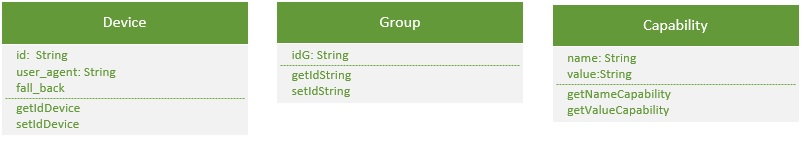
\includegraphics[width=.90\textwidth]{./imagenes/estructuras.jpg}
		\caption{Estructura de datos}
		\label{Estructura de datos}
	\end{center}
\end{figure}

Para utilizar las estructuras tuvimos que parsear el archivo de tal manera que los datos se setearan dentro de ellas por esto cada estructura tienen sus funciones getter y setter, al momento de leer el archivo de texto no se habia investigado acerca del paquete \textbf{readFile} pero una vez que se lo aprendio, lo implementamos y nos hizo mas sencillo nuestra labor con el archivo XML.\\

Luego se utilizo la función \textbf{splitOneOf} para separar al string que se obtuvo de la funcion readFile de los caracteres especiales pero nos devolvia espacios vacios innecesarios entonces esto no era como lo deseabamos, para esto implementamos una funcion que remueva estos espacios vacios la denominamos \textbf{removeEmpty} que esto por ultimo nos termino dando una lista de String que era lo que deseabamos.\\

Para trabajar con la lista de Strings lo trabajamos linea a linea, al trabajar de esa manera se procesaban cada una de las lineas que se leian en la que se distinguian por la cabecera de cada linea redirigiendolas a procesos de cada uno de los grupos.\\

Para trabajar linea a linea se utilizo diferentes funciones para cada grupo, para device se utilizo la funcion \textbf{deviceFunction} esta funcion coge a la linea que empieza con la palabra "device" y de ella saca el id del Device, user\_agent y fall\_back, caso contrario tendremos que la linea empezara con la palabra "group" se implementa la funcion \textbf{groupFunction}, esta funcion de la linea que se esta leyendo obtenemos el idGroup y por ultimo tenemos el caso en que la linea empieze con la palabra "capability" aqui utilizamos la funcion \textbf{capabilityFunction} esta funcion nos devuelve de la linea, el name y value de la capability.\\


\chapter{Observaciones}
\begin{itemize}
\item \textbf{Leonel Ramírez Gonzalez}
\begin{itemize}
	\item[Ventajas: ]Una de las ventajas que me agrado en haskell fue que al momento de leer el archivo su implementación era mas sencilla de la que se implementa en otros lenguajes.
	\item[Desventajas: ]Una de las desventajas que encontre yo de Haskell fue la manera de como se reciben los parametros en las funciones.
\end{itemize}
\item \textbf{José Vélez Gómez}
\begin{itemize}
	\item[Ventajas: ] Lo que me agrado de Haskell fue su potencial con las funciones recursivas y que incluye soporte de tipos de datos junto al manejo de listas, tuplas. Fue una herramienta de gran utilidad para implementar nuestro analizador sintactico.
	\item[Desventajas: ]Una desventaja era que como era recursivo no podiamos tener un valor guardado, entonces empleamos qeu cada vez que se mandaba a llamar la funcion recursiva le enviabamos ese valor tambien como referencia y cada vez que se llamaba la funcion, teniamos el valor, pero fue un poco complejo decifrar esa manera de tener ese valor actualizado.
\end{itemize}
\item \textbf{Kevin Campuzano Castillo}
\begin{itemize}
	\item[Ventajas: ]La ventaja que note de haskell es que no se tiene que poner en orden a las funciones, es decir es al 	libre albedrio.
	\item[Desventajas: ] Una de las desventajas para mi fue la forma en la que se debe de recorrer listas en este 		lenguajes, es mas complicado que en otros lenguajes.
\end{itemize}
\end{itemize}
\end{document}